\section{The Data}

The dataset consists of 3345 root comments from Reddit and Facebook, and there’s an uncounted number of root tweets, since these were automatically split from comments into sentences by the script that extracted them. The 3345 comments was collected from 239 different articles that were spread on 92 different tags/topics. All together this yielded us 9008 labelled sentences of which 51\% is from Facebook, 27.6\% is from Reddit and 21.4\% is from Twitter: 

\begin{figure}[H]
	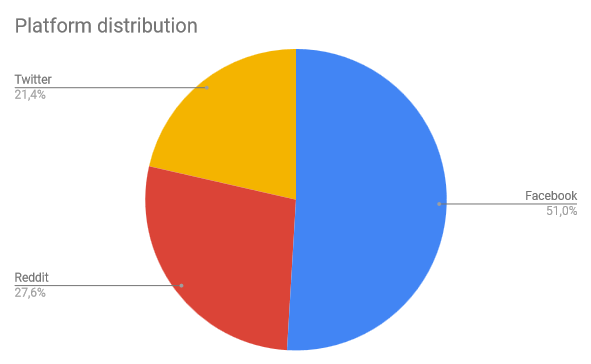
\includegraphics[width=0.5\textwidth]{Images/DataSetConsistsOf}
	\centering
	\caption{Distribution of sentences on social media}
	\label{datastats}
\end{figure}

Of the 9008 sentences there are 1489 positive, 4057 neutral and 3462 negatives, which is 16\%, 45\% and 39\% of the whole dataset respectively, and gives us around 22\% more negatives than positives.  A figure of the statistics of these statistics can be seen on figure \ref{datastats}. And there is no surprise here since it’s commonly known that there’s a higher chance of people with negative sentiment will express their opinions. \cite{marketing}

\begin{figure}[H]
	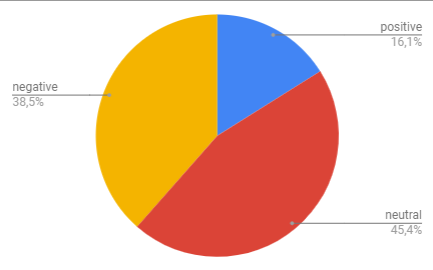
\includegraphics[width=0.5\textwidth]{Images/DataStats}
	\centering
	\caption{Distribution of our classes.}
	\label{datastats}
\end{figure}

One thing that came as a surprise - though it make perfect sense - was the deviation of sentiment across the social media platforms, as seen on figure \ref{platforms}.

\begin{figure}[H]
	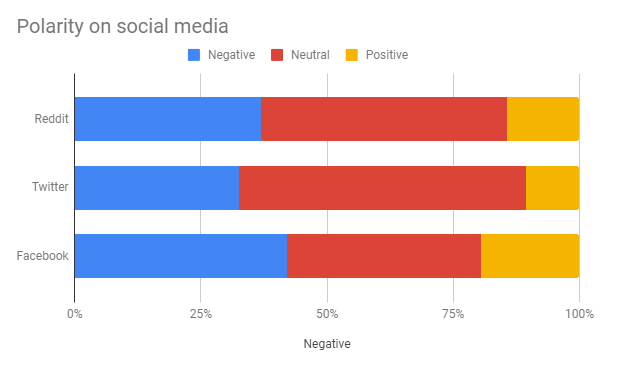
\includegraphics[width=0.5\textwidth]{Images/PlatformsCompared}
	\centering
	\caption{Comparison of sentiment across medias.}
	\label{platforms}
\end{figure}

It’s quite clear that Twitter is the most neutral of the three platforms while Reddit is not far behind; however, the surprise is that Facebook actually has more negative sentiment than neutral. There could be many reasons for this, where some individually or together may be: 
\begin{itemize}
	\item Media focuses on negative news, because they get more exposure, which then in return spawns more negative sentiment.
	\item Facebook is the much larger platform and the average person just seek to express their opinion, and those who seek to discuss it go to another platform such as Reddit.
	\item Political subjects raises negative sentiment in general, and since the exposure on Facebook is far greater than the two other platforms, the general populations sentiment/opinion is clearer.
\end{itemize}

An initial hypothesis was also that Reddit - known for being better at discussions than Facebook - should have a higher average sentence count than Facebook. To no surprise we found that Facebook only had an average sentence per comment of 1.88 whilst Reddit had 68\% more with 2.74 sentences per comment. We believe this is to be expected since well-minded discussions often provide well-formulated and longer arguments when people are discussing their views rather than just expressing them. An observation that supports this claim is that Facebook and Twitter, when seen as a whole text-document, only has a Lix-number of 25.07 whilst Reddit has 29.18. A lix-number indicates how hard a text is to read by for example accounting for long words(7 letters or more) \cite{lix}. Another observation that support this claim is that Reddit had 54 different articles with 54 different topics, while Facebook with 185 different articles only had 38 different topics.


A slight surprise was in our word frequency. Our word frequency is noticeably different from those of the written language in different aspects: Looking at table \ref{sprogetdk}, which contains our 10 most frequent words and four frequency lists from sproget.dk\cite{sprogetdk}, we see that the word "er" is not even present in the frequency list of Lemma 5000. It is less commonly used in the dictionary, in newspapers and in novels. We do think it relates to the nature of the social media platform, but we do not have concise evidence to support this claim. Our rationale is that the word "er" is often used to express a subjective opinion, and the comment section is a place of expressing subjective opinions, which consequently means the frequency list will be different from that of the common written language. This hypothesis is somewhat supported by the fact that the lix-number of our dataset combined is around 26.1~, which gives a slight indication of the comments being more akin to spoken language than written language.

\begin{table}[H]
	\centering
	\caption{Danish word frequency lists.}
	\begin{tabular}{lccccc}
		\hline
		& \multicolumn{1}{l}{Our Dataset} & \multicolumn{1}{l}{Dictionary\cite{sprogetdk}} & \multicolumn{1}{l}{Newspapers\cite{sprogetdk}} & \multicolumn{1}{l}{Novels\cite{sprogetdk}} & \multicolumn{1}{l}{Lemma 5000\cite{sprogetdk}} \\ \hline
		1  & er                              & og                                                              & i                                                               & og                                                          & i                                                               \\
		2  & det                             & i                                                               & og                                                              & det                                                         & være                                                            \\
		3  & at                              & at                                                              & at                                                              & i                                                           & og                                                              \\
		4  & og                              & det                                                             & af                                                              & at                                                          & en                                                              \\
		5  & i                               & er                                                              & er                                                              & han                                                         & den                                                             \\
		6  & ikke                            & en                                                              & en                                                              & var                                                         & på                                                              \\
		7  & en                              & på                                                              & til                                                             & jeg                                                         & til                                                             \\
		8  & der                             & til                                                             & det                                                             & en                                                          & det                                                             \\
		9  & de                              & med                                                             & for                                                             & ikke                                                        & at                                                              \\
		10 & til                             & af                                                              & der                                                             & til                                                         & af                                                              \\ \hline
	\end{tabular}
	\label{sprogetdk}
\end{table}
